\subsection{问题二的模型建立与求解}

问题二的核心目标是,针对接受无创产前检测(NIPT)的孕妇,依据其身体质量指数(BMI)进行合理分组,并为每个分组推荐一个最佳的检测时点(以孕周计)。这一策略旨在最小化因检测时点选择不当而引发的综合风险,例如过早检测导致的失败率增高,或因推迟检测而错过了最佳干预时机。

为实现此目标,我们构建了一个从概率建模到优化决策的完整分析框架。首先,我们建立一个概率模型来预测在不同BMI和孕周条件下,Y染色体浓度检测的达标可能性。其次,我们定义一个能够量化潜在风险的期望风险函数。最后,通过优化算法,我们寻找能够使全体孕妇总期望风险最小化的BMI分组方案与相应的推荐检测周。

\subsubsection{模型基础:基于样条回归的达标概率预测}

为了精确描述Y染色体浓度是否达标与孕妇生理特征(尤其是BMI和孕周)之间的复杂关系,我们构建了一个基于改进样条回归的概率预测模型。该模型直接对"是否达标"这一二元结果进行建模,能够有效捕捉非线性趋势。

\paragraph{1. 特征工程与模型设定}
模型的预测效果在很大程度上依赖于特征的构造。我们引入了样条特征来增强模型的表达能力,具体包含了以下部分:
\begin{itemize}
    \item \textbf{基础线性项}:涵盖了标准化处理后的BMI、孕周和年龄。
    \item \textbf{高次项与交互项}:为捕捉变量间的非线性关系,我们加入了$\text{BMI}^2$、$\text{孕周}^2$以及BMI与孕周的交互项(BMI $\times$ 孕周)。
    \item \textbf{二次样条项}:为了更灵活地拟合局部变化趋势,我们分别为BMI和孕周设置了二次样条,形式为$\max(0, \text{变量} - k)^2$,其中$k$是根据数据分位数确定的节点。
\end{itemize}

\paragraph{2. 正则化逻辑回归}
在构建好特征矩阵$\mathbf{X}$后,我们采用带弹性网络正则化(Elastic Net)的逻辑回归模型来拟合达标概率$p$。其基本形式为:
\begin{equation}
    \log\left(\frac{p}{1-p}\right) = \mathbf{X}\boldsymbol{\beta}
\end{equation}
模型的优化目标是在最小化负对数似然损失的同时,对系数$\boldsymbol{\beta}$施加L1和L2范数惩罚,其目标函数如下:
\begin{equation}
    \min_{\boldsymbol{\beta}} \left\{ -\sum_{i=1}^n \left[ y_i \log p_i + (1-y_i) \log(1-p_i) \right] + \lambda_1 \|\boldsymbol{\beta}\|_1 + \lambda_2 \|\boldsymbol{\beta}\|_2^2 \right\}
\end{equation}
这种方法不仅能自适应地捕捉数据中的非线性模式,还能通过正则化有效防止模型过拟合,为后续的风险评估与优化决策提供了稳健的概率预测基础。

我们通过ROC曲线对模型性能进行了评估,其AUC值为0.693,表明该概率模型具有良好的分类预测能力。图~\ref{fig:qualification_probability}直观展示了达标概率在BMI-孕周平面上的分布情况,清晰地揭示了达标可能性随这两个核心变量的变化趋势。

\subsubsection{期望风险最小化模型}

为了对检测时点选择的优劣进行量化评估,我们构建了一个期望风险模型。

\paragraph{1. 风险函数的定义}
我们认为,检测时点带来的风险并非线性增加,也非阶梯式跳跃。因此,我们设计了一个平滑的二次函数来描述风险随检测时点$T$的变化。该函数在孕周11周前风险为最低值$R_{\min}$,在28周后达到最高值$R_{\max}$,中间则平滑过渡。其数学表达式为:
\begin{equation}
    R(T) = 
    \begin{cases} 
        R_{\min} & \text{if } T \le 11 \\
        R_{\min} + a(T - 11)^2 & \text{if } 11 < T < 28 \\
        R_{\max} & \text{if } T \ge 28 
    \end{cases}
\end{equation}
其中,$R_{\min} = 1.0$,$R_{\max} = 30.0$,$a = \frac{R_{\max} - R_{\min}}{(28-11)^2}$。这样的设计既符合风险随时间推移而加速增长的临床直觉,也保证了函数在边界点的连续性,有利于后续的数值优化。

\paragraph{2. 增强的期望风险函数}
传统的期望风险模型通常只考虑检测成功的情况。我们对其进行了改进,引入了检测失败的惩罚机制。对于一位特定BMI的孕妇,在孕周$T$进行检测的期望风险$E(T | \text{BMI})$被定义为:
\begin{equation}
    E(T | \text{BMI}) = p(\text{BMI}, T) \cdot R(T) + (1 - p(\text{BMI}, T)) \cdot [R(T+k) + P_{\text{failure}}]
\end{equation}
此处的$p(\text{BMI}, T)$是由前述样条回归模型预测的达标概率。当检测成功(概率为$p$)时,风险为$R(T)$;当检测失败(概率为$1-p$)时,孕妇不仅要承担下一次检测(假设在$k$周后)的风险$R(T+k)$,还需承受一个额外的失败惩罚$P_{\text{failure}}$(我们设定$k=2$周,$P_{\text{failure}}=10.0$)。这个增强模型更真实地反映了检测失败所带来的时间、经济和心理等多重代价,使优化过程更倾向于选择成功率高且时间较早的检测方案。

图~\ref{fig:expected_risk_heatmap}通过热力图的形式,展示了期望风险在BMI与孕周构成的二维平面上的分布,为后续寻找最优策略提供了直观依据。

\begin{figure}[htbp]
    \centering
    \begin{minipage}{0.48\textwidth}
        \centering
        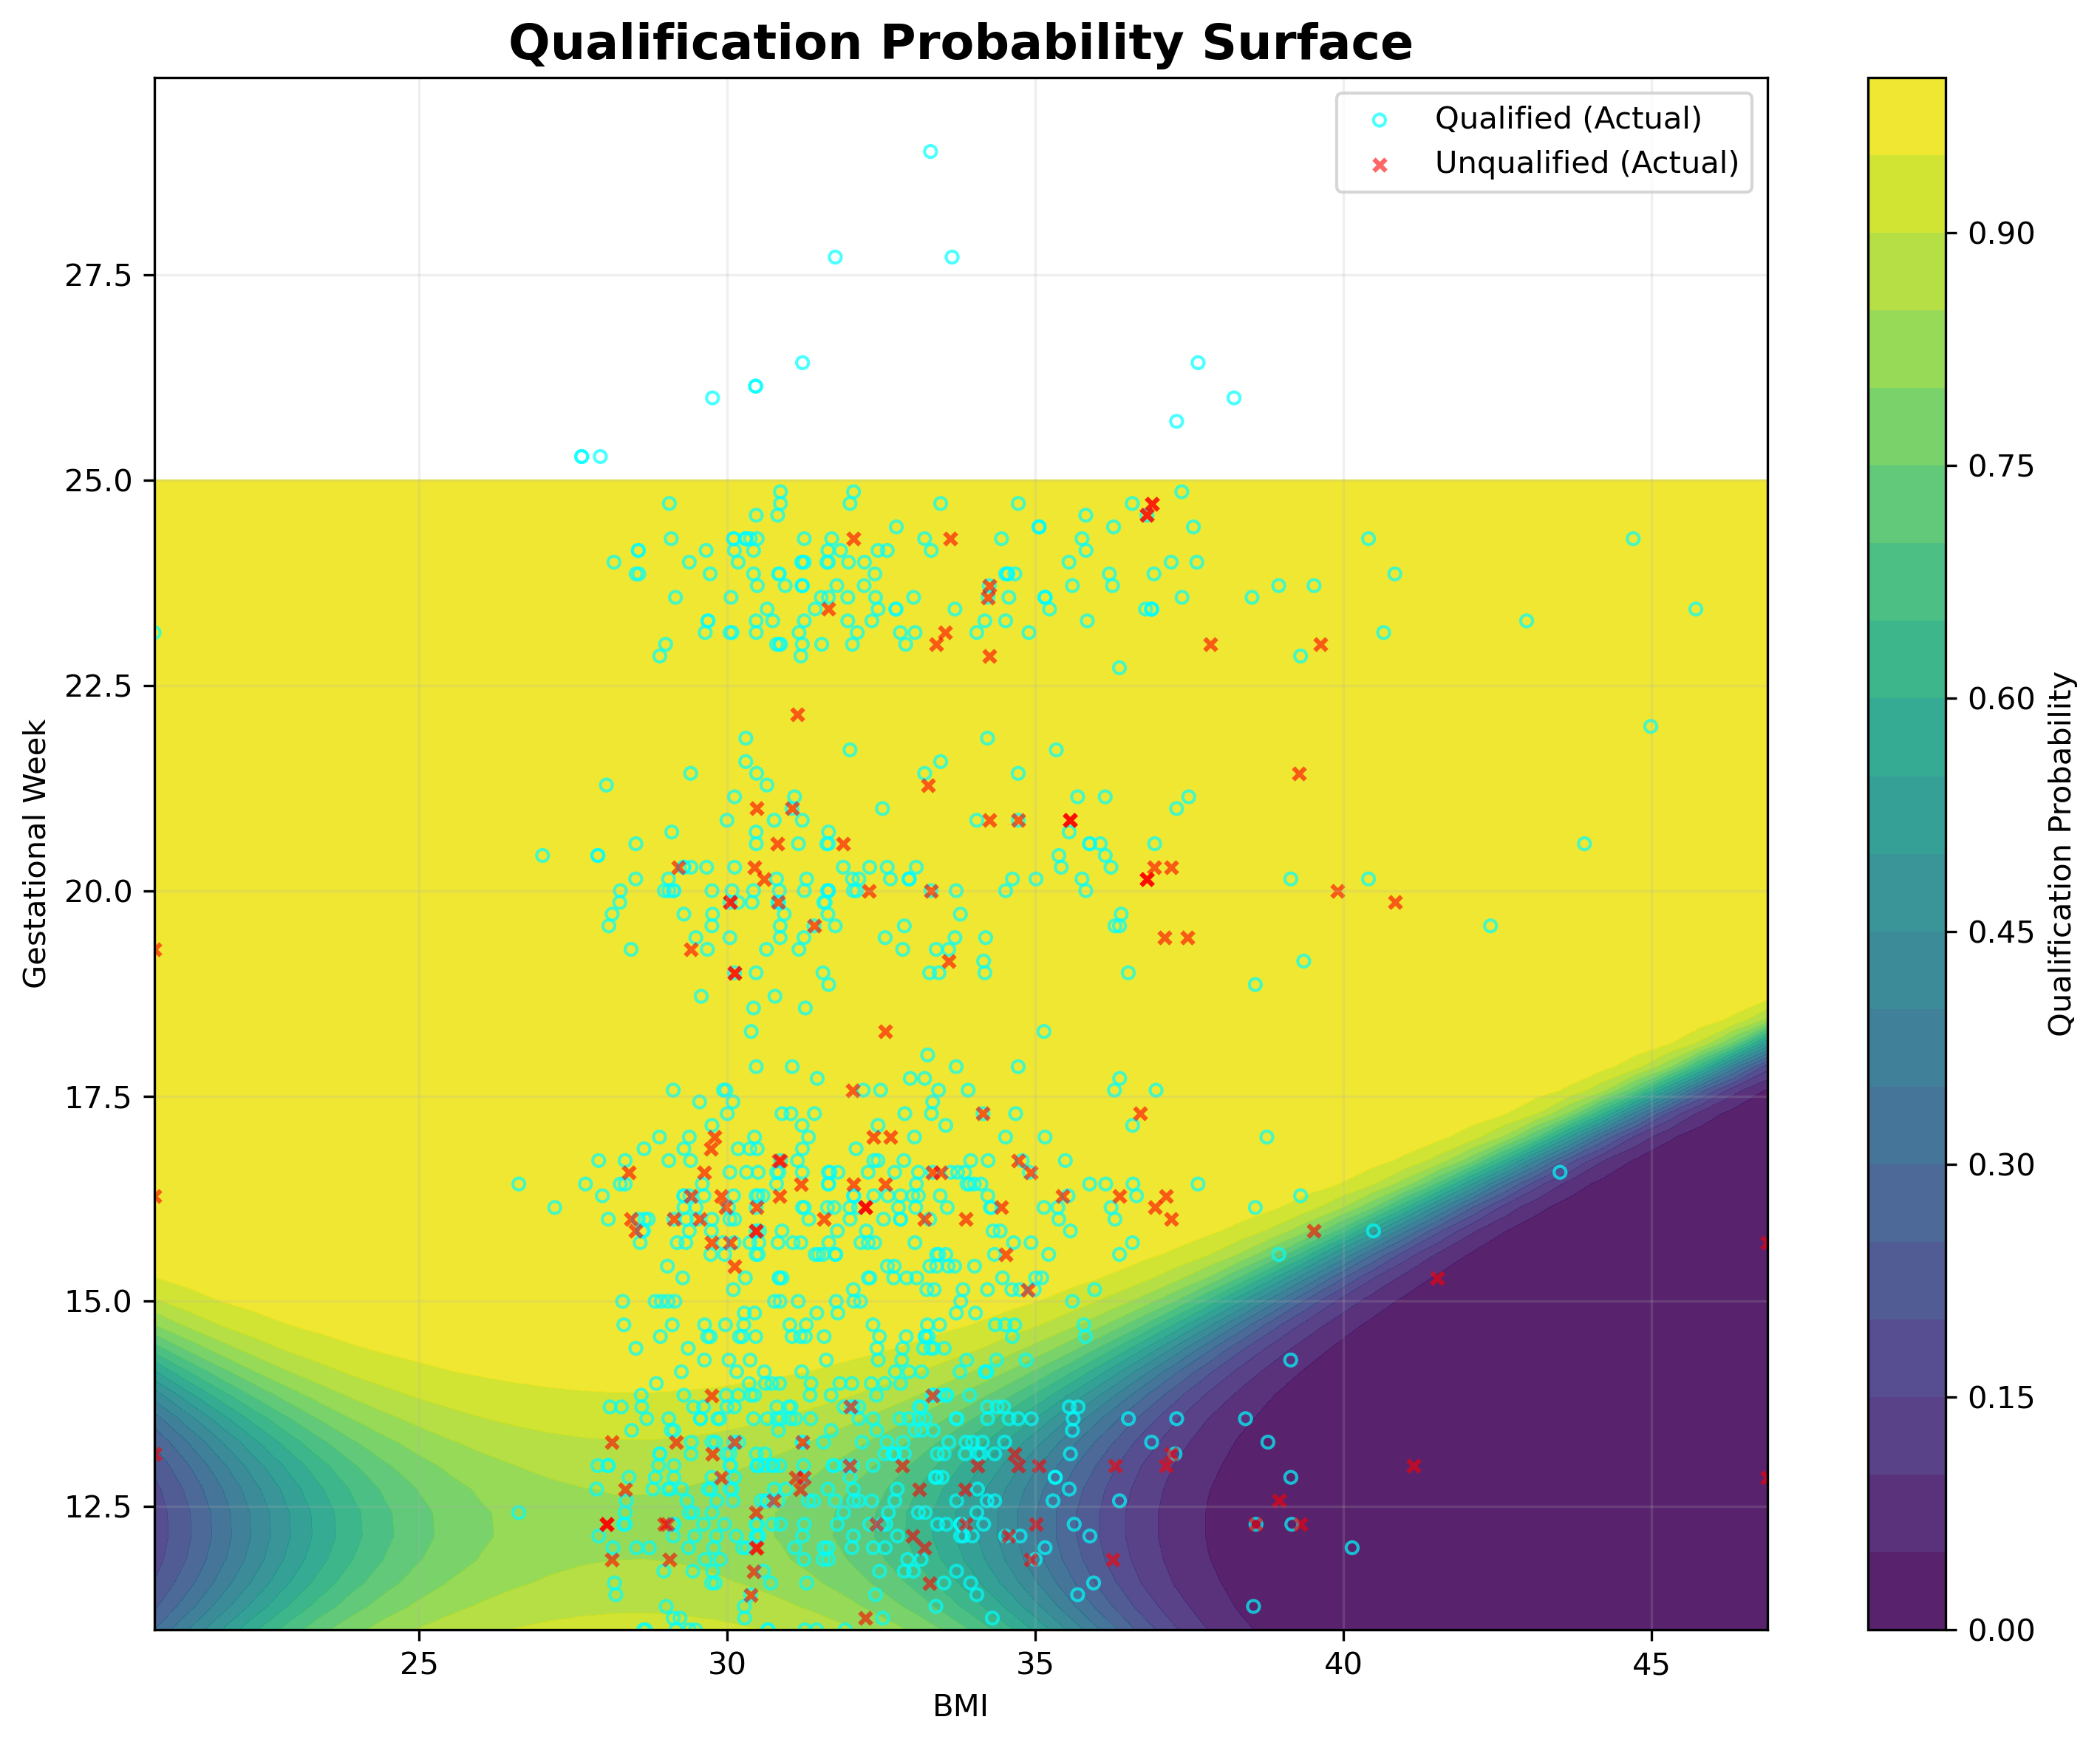
\includegraphics[width=\textwidth]{q2/qualification_probability_surface.png}
        \caption{Y染色体浓度达标概率等高图}
        \label{fig:qualification_probability}
    \end{minipage}
    \hfill
    \begin{minipage}{0.48\textwidth}
        \centering
        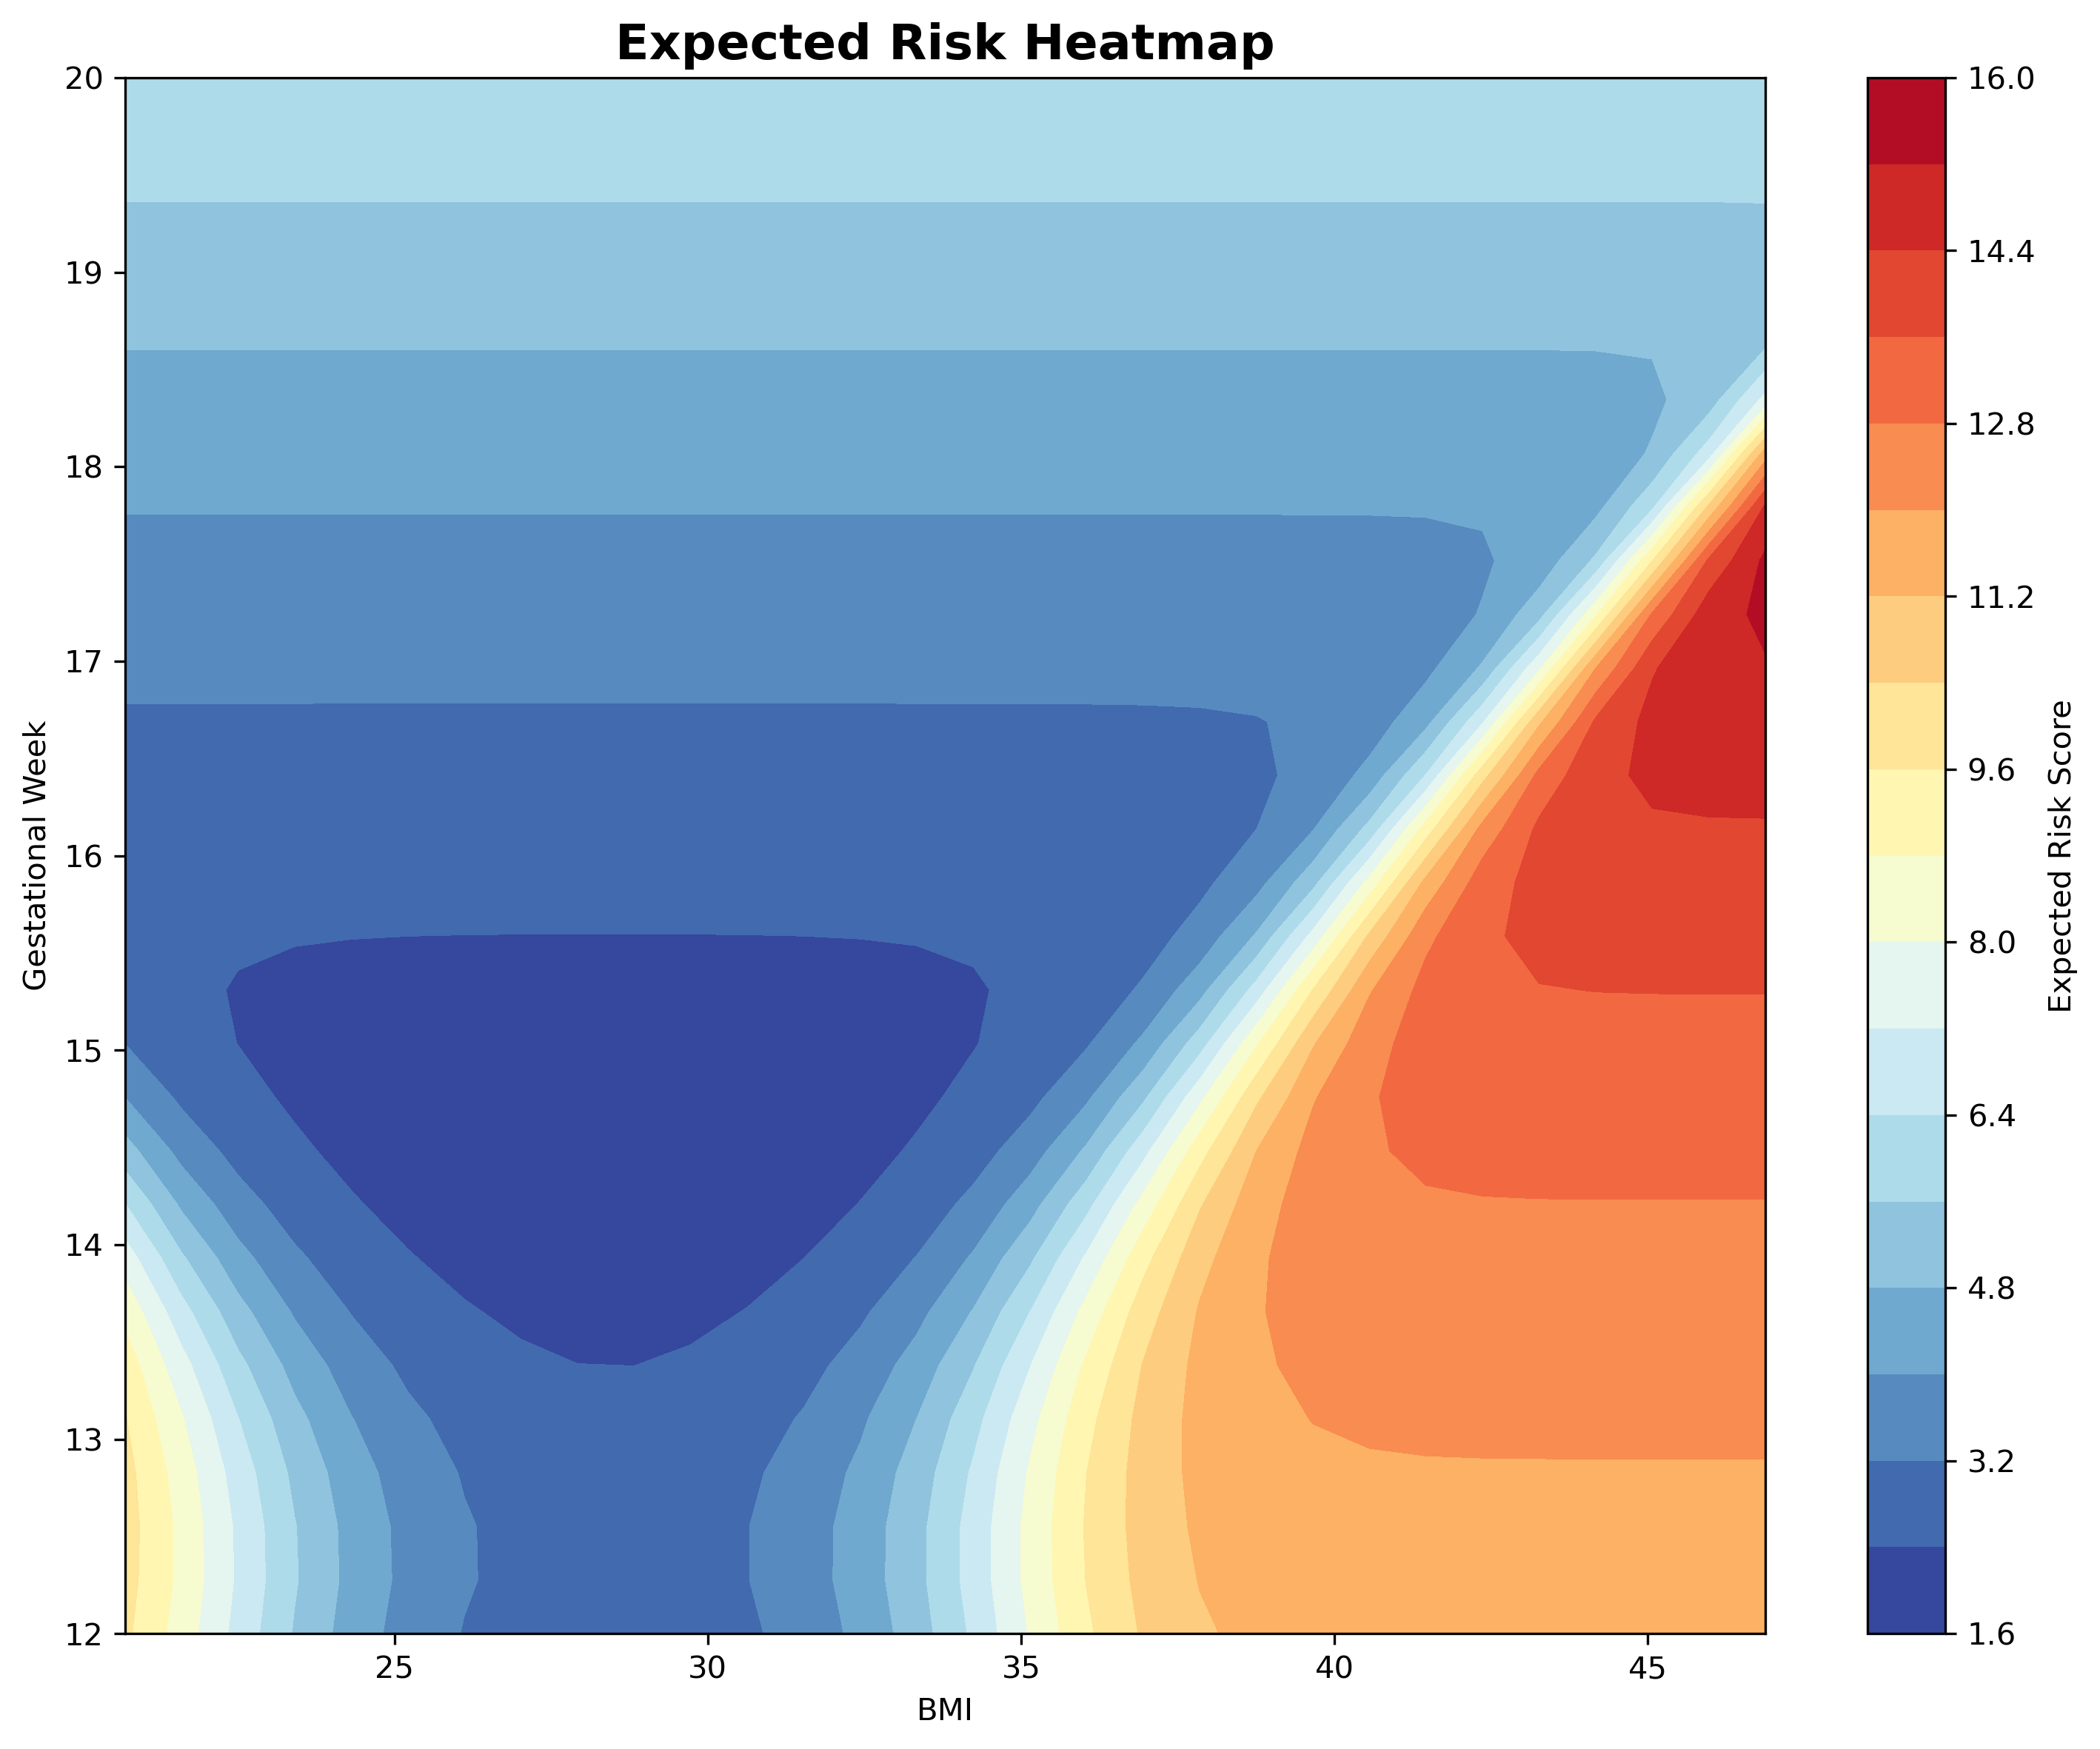
\includegraphics[width=\textwidth]{q2/expected_risk_heatmap.png}
        \caption{BMI-孕周期望风险热力图}
        \label{fig:expected_risk_heatmap}
    \end{minipage}
\end{figure}

\subsubsection{最优分组与时点选择策略}

我们的最终目标是寻找一个最优的BMI分组方案 $\{G_1, G_2, \dots, G_N\}$,并为每个组 $G_i$ 确定一个统一的最佳检测时点 $T_i^*$,以实现所有孕妇总期望风险的最小化。

\paragraph{1. 优化目标}
对于一个给定的分组方案,每个组 $G_i$ 的最佳检测时点 $T_i^*$ 应是使该组内所有个体期望风险之和最小的周数:
\begin{equation}
    T_i^* = \arg\min_{T} \sum_{j \in G_i} E(T | \text{BMI}_j)
\end{equation}
而我们的全局优化目标,则是找到能使所有组的总风险之和最小的分组方案本身:
\begin{equation}
    \min_{\{G_1, \dots, G_N\}} \sum_{i=1}^{N} \left( \sum_{j \in G_i} E(T_i^* | \text{BMI}_j) \right)
\end{equation}

\paragraph{2. 求解算法}
这是一个复杂的混合优化问题。我们采用了一致性的优化思想,即分组边界的确定与各组最佳时点的选择应在同一个目标函数下进行。具体实现上,我们利用\textbf{基于梯度的优化算法(如L-BFGS-B)}来高效地寻找能够最小化全局期望风险的BMI分割点。在算法的每次迭代中,我们都会同步计算当前分组方案下的最优检测时点,从而保证了分组决策与时点选择的理论一致性,有效规避了局部最优陷阱。为确保结果的稳健性,我们还对分割点的搜索范围进行了合理约束,避免产生样本量过小的分组。

\subsubsection{检测误差对结果影响的分析}

为了评估现实中可能存在的检测误差对我们模型决策稳定性的影响,我们设计并实施了敏感性分析。

\paragraph{1. 误差建模与模拟}
我们认为,检测误差对决策的影响主要体现在Y染色体浓度值接近4\%临界点的样本上。因此,我们重点关注此关键区域(4\% ± 0.5\%)内的样本,该区域共包含89个样本。我们采用相对误差模型来描述检测中的不确定性,即假定观测值$C_{\text{observed}}$是在真实值$C_{\text{true}}$的基础上乘以一个服从正态分布的随机扰动项$1 + \epsilon$,其中$\epsilon \sim N(0, (\text{CV})^2)$,CV为测量变异系数。

基于此模型,我们通过并行化的蒙特卡洛模拟来执行敏感性分析。在每次模拟中,我们对关键区域内的样本添加随机误差,重新训练概率模型,并再次执行完整的分组优化过程。通过重复此过程,我们得以统计BMI分割点和推荐检测时点在多次模拟中的波动情况。

\paragraph{2. 稳定性评估}
我们通过计算各参数(BMI分割点、推荐检测时点)在多次模拟结果中的标准差等统计量,来定量评估模型的稳定性。这能够帮助我们判断,在存在一定检测误差的情况下,我们提出的分组策略是否依然可靠。

\subsubsection{模型求解与结果分析}

我们将上述理论框架应用于所给的男胎孕妇数据。

\paragraph{1. 数据与模型训练}
经过数据清洗与预处理后,我们共得到1081个有效样本,其中达标样本936个,总体达标率为86.6\%。样本的BMI范围为20.7至46.9,孕周范围为11.0至29.0周。基于这些数据训练的样条回归模型,其准确率约为86.4\%,AUC值达到0.693,表现出良好的预测性能。

\paragraph{2. 模型验证与特征分析}
为进一步验证模型的稳健性与关键影响因素,我们采用了随机森林模型进行5折交叉验证。结果显示,模型的泛化性能良好,且特征重要性分析表明,BMI是影响达标概率的最主要因素(重要性占比约51\%),其次是检测孕周(约31\%)和年龄(约18\%)。这一发现为我们后续以BMI为核心进行分组的策略提供了有力的数据支持。

\paragraph{3. 最优分组结果}
通过我们的一致性优化算法,得到的最优BMI分组方案如表~\ref{tab:optimal_grouping}所示。该方案将孕妇分为四个BMI组,并为每个组提供了具体的推荐检测时点和对应的平均期望风险。

\begin{table}[htbp]
\centering
\caption{最优BMI分组方案与推荐检测时点}
\label{tab:optimal_grouping}
\begin{tabular}{ccccc}
\toprule
分组 & BMI范围 & 样本数 & 推荐检测时点(周) & 期望风险评分 \\
\midrule
1 & [20.7, 30.5) & 343 & 14.7 & 2.368 \\
2 & [30.5, 33.6) & 431 & 14.2 & 2.358 \\
3 & [33.6, 37.6) & 259 & 14.4 & 2.520 \\
4 & [37.6, 46.9) & 48 & 15.6 & 3.411 \\
\bottomrule
\end{tabular}
\end{table}

图~\ref{fig:bmi_distribution}与图~\ref{fig:bmi_week_heatmap}分别从BMI一维分布和BMI-孕周二维平面的角度,直观地展示了最优分组边界和推荐策略。

\begin{figure}[htbp]
    \centering
    \begin{minipage}{0.48\textwidth}
        \centering
        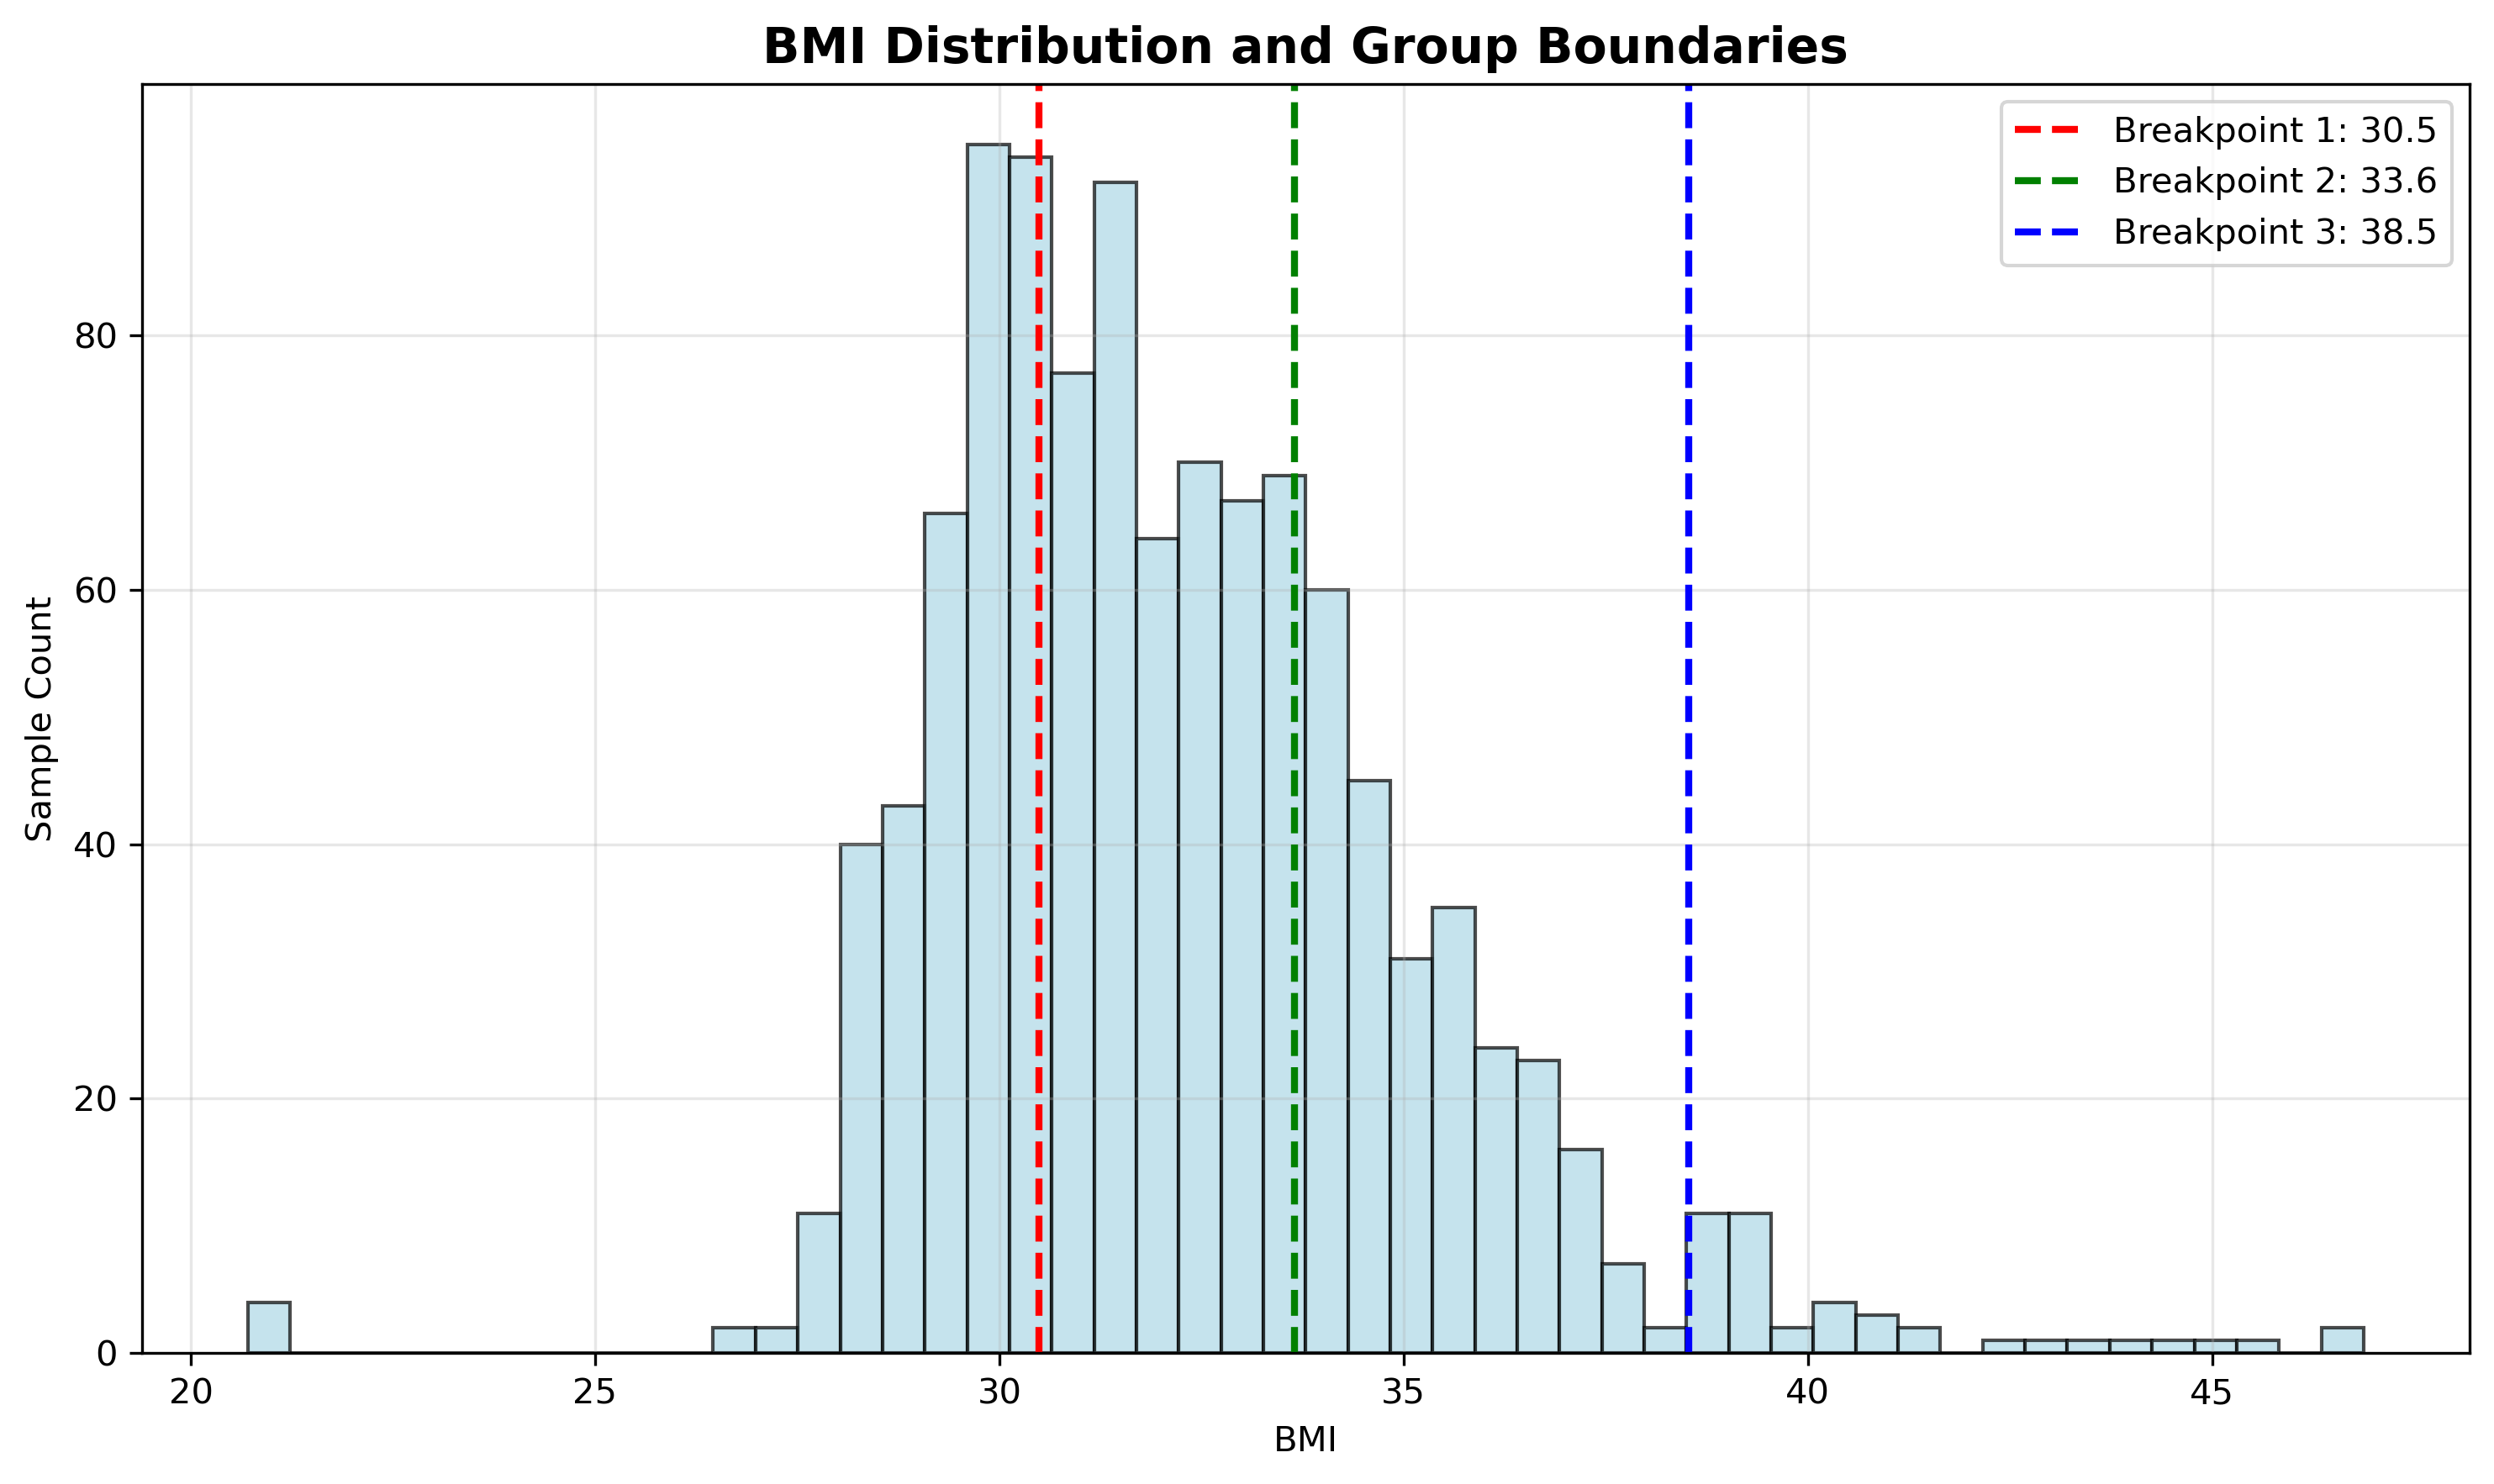
\includegraphics[width=\textwidth]{q2/bmi_distribution_with_boundaries.png}
        \caption{BMI分布与分组边界}
        \label{fig:bmi_distribution}
    \end{minipage}
    \hfill
    \begin{minipage}{0.48\textwidth}
        \centering
        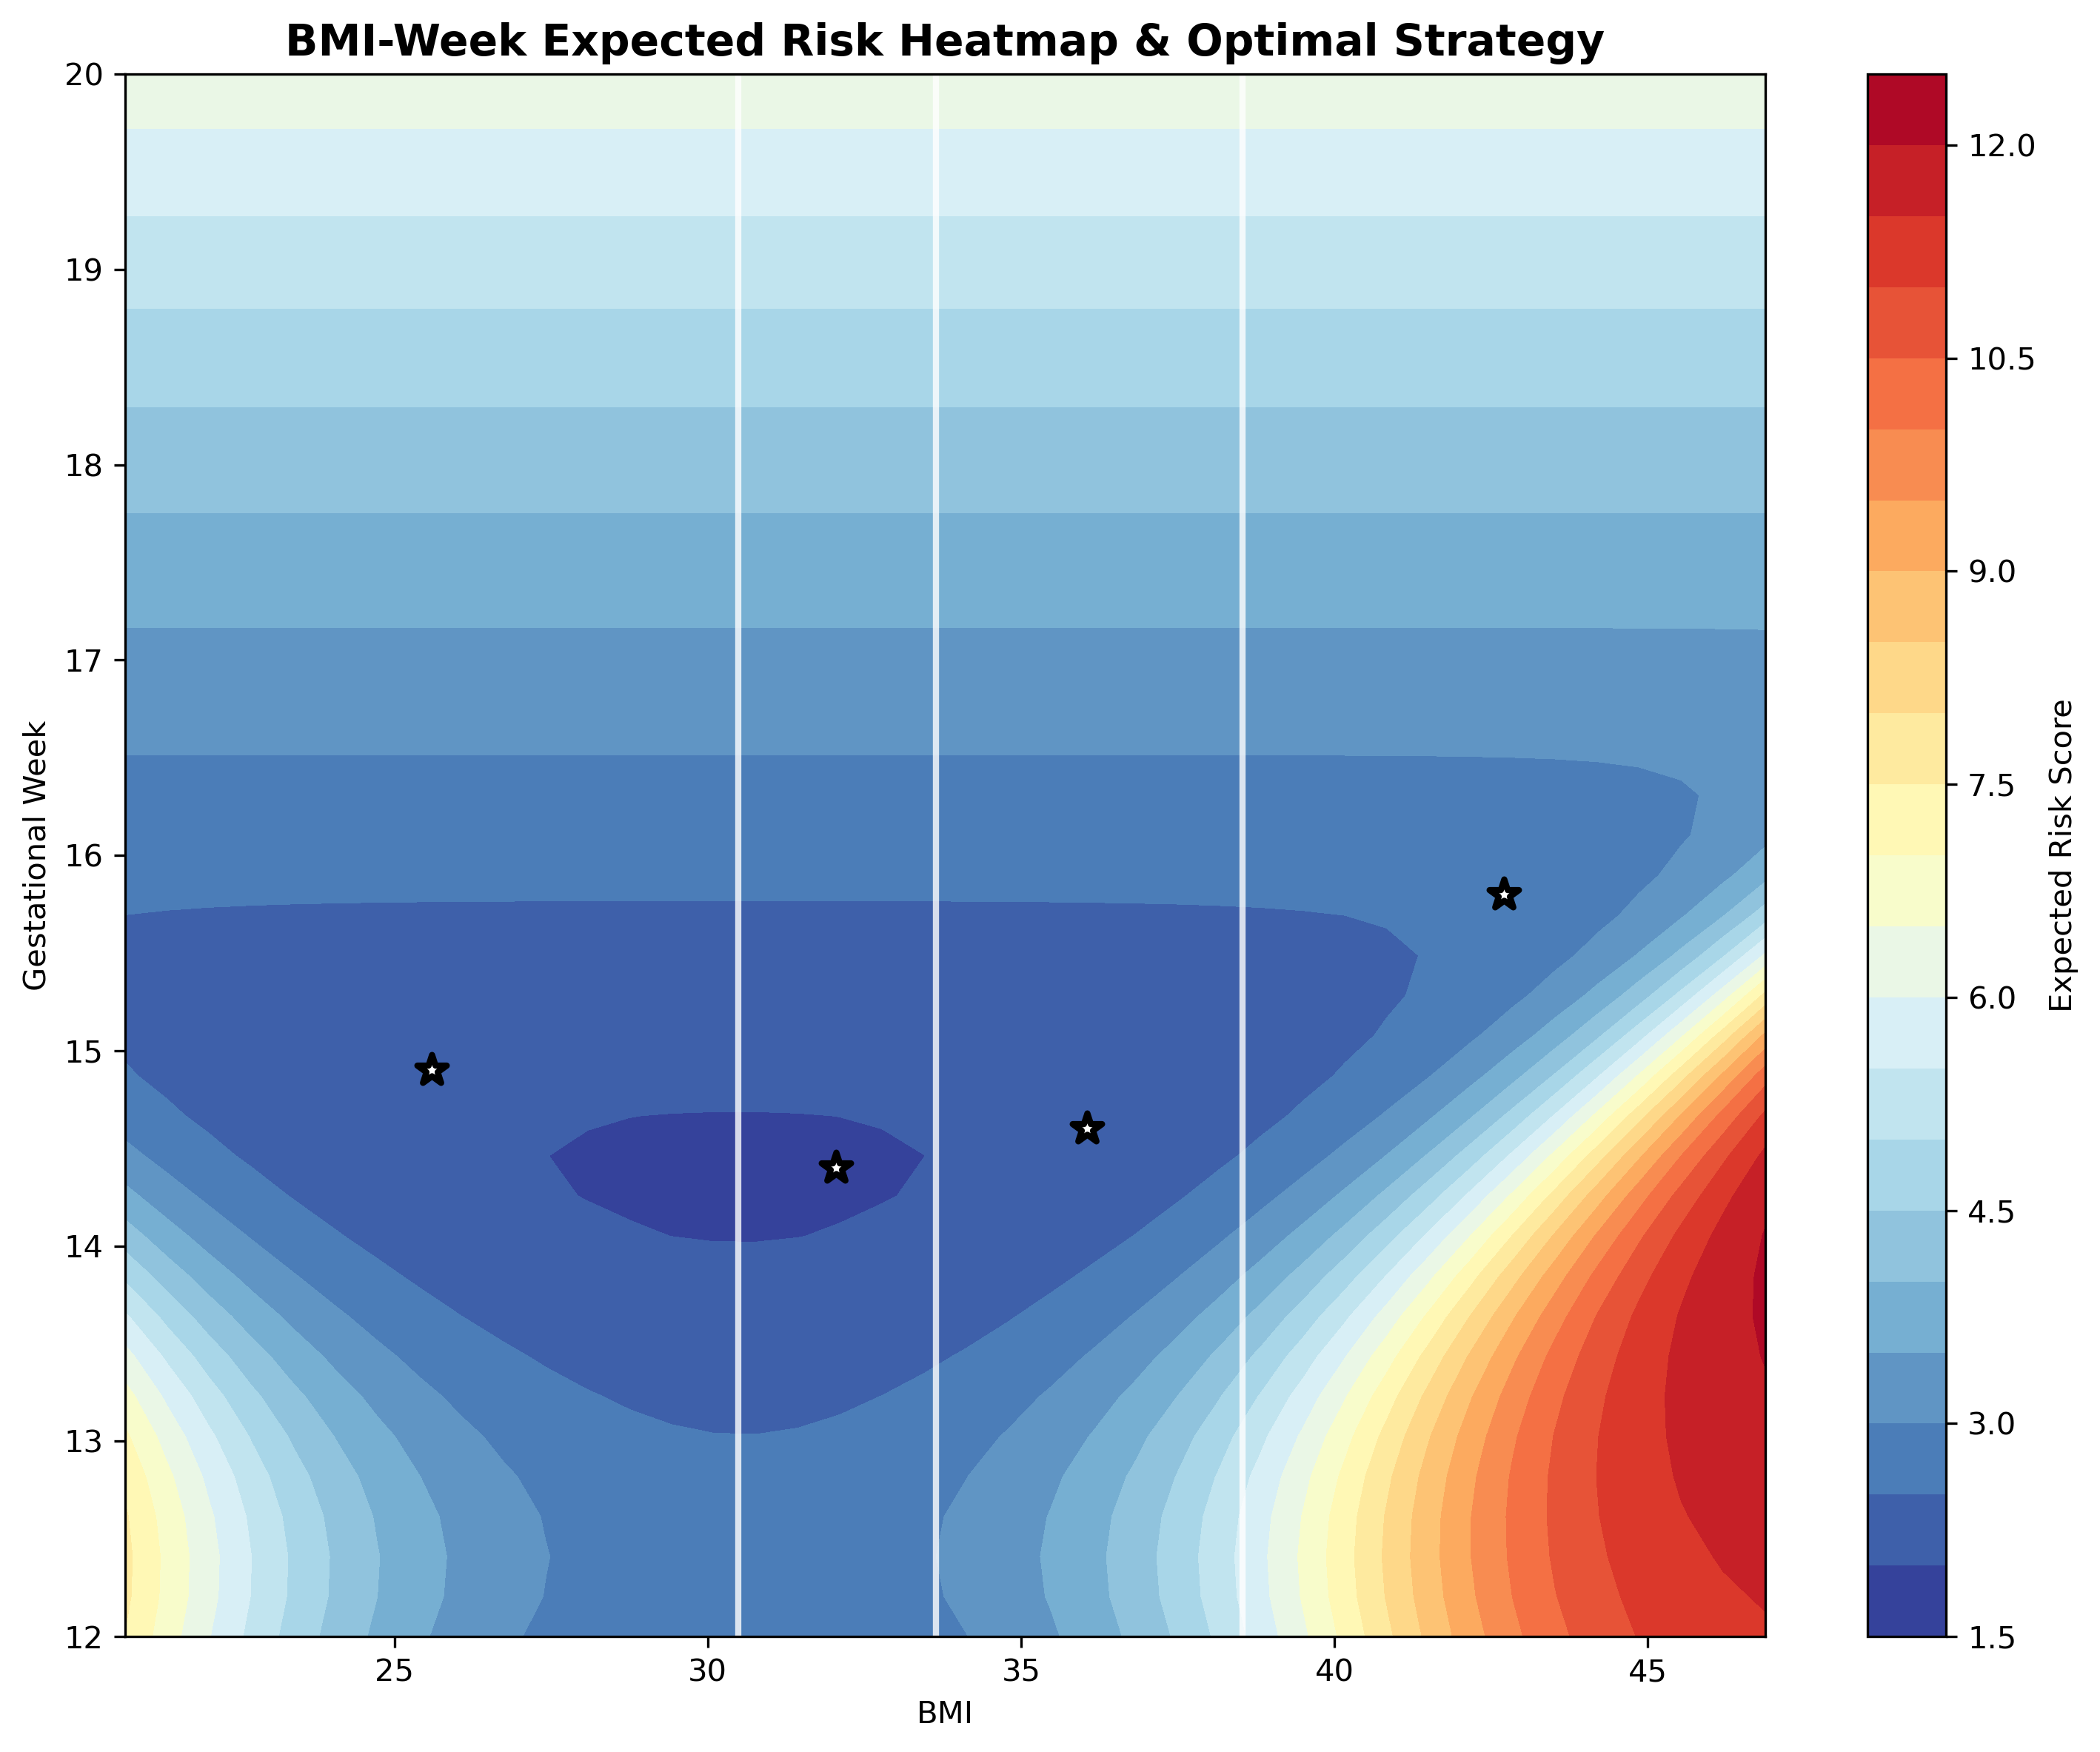
\includegraphics[width=\textwidth]{q2/bmi_week_risk_heatmap.png}
        \caption{BMI-孕周期望风险热力图与最优策略}
        \label{fig:bmi_week_heatmap}
    \end{minipage}
\end{figure}

\paragraph{4. 敏感性分析结果}
我们设定测量变异系数为15\%,对模型进行了30次蒙特卡洛模拟。结果如表~\ref{tab:sensitivity_analysis}所示。

\begin{table}[htbp]
\centering
\caption{敏感性分析结果:分割点和推荐时点的稳定性}
\label{tab:sensitivity_analysis}
\begin{tabular}{lccc}
\toprule
参数类型 & 参数名称 & 标准差 & 稳定性评估 \\
\midrule
\multirow{3}{*}{BMI分割点} & 分割点1 (30.4) & 0.561 & 较为稳定 \\
                         & 分割点2 (33.6) & 0.292 & 高度稳定 \\
                         & 分割点3 (38.4) & 1.564 & 一般 \\
\midrule
\multirow{4}{*}{推荐检测时点} & 分组1时点 (14.7周) & 0.116 & 高度稳定 \\
                            & 分组2时点 (13.9周) & 0.673 & 较为稳定 \\
                            & 分组3时点 (13.9周) & 1.184 & 一般 \\
                            & 分组4时点 (15.1周) & 1.747 & 一般 \\
\bottomrule
\end{tabular}
\end{table}

\begin{figure}[htbp]
    \centering
    \begin{minipage}{0.48\textwidth}
        \centering
        \includegraphics[width=\textwidth]{q2/sensitivity_breakpoints_stability.png}
        \caption{BMI分割点稳定性分析}
        \label{fig:sensitivity_breakpoints}
    \end{minipage}
    \hfill
    \begin{minipage}{0.48\textwidth}
        \centering
        \includegraphics[width=\textwidth]{q2/sensitivity_weeks_stability.png}
        \caption{推荐检测时点稳定性分析}
        \label{fig:sensitivity_weeks}
    \end{minipage}
\end{figure}

分析发现,中低BMI范围的分组边界和推荐时点表现出高度的稳定性,而高BMI分组的参数则受误差影响较大,这可能是因为该分组的样本量较少。如图~\ref{fig:sensitivity_breakpoints}和图~\ref{fig:sensitivity_weeks}所示,敏感性分析的可视化结果进一步验证了这一发现。尽管如此,核心的分组策略在存在15\%测量变异系数的情况下依然保持了相对稳定,证明我们提出的模型和策略具有良好的鲁棒性和实际应用价值,能够为临床NIPT检测提供科学可靠的决策支持。